\documentclass[12pt]{article}
\usepackage[utf8]{inputenc}
\usepackage{float}
\usepackage{amsmath}


\usepackage[hmargin=3cm,vmargin=6.0cm]{geometry}
%\topmargin=0cm
\topmargin=-2cm
\addtolength{\textheight}{6.5cm}
\addtolength{\textwidth}{2.0cm}
%\setlength{\leftmargin}{-5cm}
\setlength{\oddsidemargin}{0.0cm}
\setlength{\evensidemargin}{0.0cm}

%misc libraries goes here
\usepackage{tikz}
\usetikzlibrary{automata,positioning}

\begin{document}

\section*{Student Information } 
%Write your full name and id number between the colon and newline
%Put one empty space character after colon and before newline
Full Name : Beyazıt Yalçınkaya \\
Id Number : 2172138 \\

% Write your answers below the section tags
\section*{Answer 1}

\subsection*{a.}
Let's denote the set of rational numbers inside the open interval $(-1, 0)$ as $S$ and elements of $S$ as $\dfrac{a}{b}$ where $a \in \mathbf{Z}^{-}$ and $b \in \mathbf{Z}^{+}$. \\
Note that, say $\alpha, \beta \in \mathbf{Z}^{+}$, then $\dfrac{\alpha}{\beta}$ is a positive rational number. When this positive rational number is multiplied by $-1$, it becomes the negative rational number $-\dfrac{\alpha}{\beta}$. For this negative rational  number it follows that $-\dfrac{\alpha}{\beta} = \dfrac{-\alpha}{\beta} = \dfrac{\alpha}{-\beta}$, since $\alpha, \beta \in \mathbf{Z}^{+}$ and $(-1) \times \dfrac{\alpha}{\beta} = \dfrac{(-1) \times \alpha}{\beta} = \dfrac{\alpha}{(-1) \times \beta}$. Thus, the proof that will be constructed will hold regardless of the assumptions made for the integers $a$ and $b$, meaning choosing $a$ to be a negative integer and $b$ to be a positive integer does not change the proof, vice versa could have been chosen as well. \\
Since $a \in \mathbf{Z}^{-}$ and $b \in \mathbf{Z}^{+}$ and both $\mathbf{Z}^{-}$ and $\mathbf{Z}^{+}$ are infinite sets, there is no $n$ such that $S$ is equinumerous with the set $\{1, 2, 3, 4, ..., n\}$ for $n \in \mathbf{N}$. Thus, $S$ is not a finite set, it follows that $S$ is an infinite set.\\
For the set of rational numbers that can be obtained from $a$ and $b$, the following table can be constructed.

\begin{table}[H]
        \caption{}
        \begin{center}
        \begin{tabular}{ c | c c c c c c }
                      & $1$ & $2$ & $3$ & $4$ & $5$ & $...$ \\
                \hline &&&&&&\\
                $-1$ & $\dfrac{-1}{1}$ & $\dfrac{-1}{2}$ & $\dfrac{-1}{3}$ & $\dfrac{-1}{4}$ & $\dfrac{-1}{5}$ & $...$  \\&&&&&&\\
                $-2$ & $\dfrac{-2}{1}$ & $\dfrac{-2}{2}$ & $\dfrac{-2}{3}$ & $\dfrac{-2}{4}$ & $\dfrac{-2}{5}$ & $...$  \\&&&&&&\\
                $-3$ & $\dfrac{-3}{1}$ & $\dfrac{-3}{2}$ & $\dfrac{-3}{3}$ & $\dfrac{-3}{4}$ & $\dfrac{-3}{5}$ & $...$  \\&&&&&&\\
                $-4$ & $\dfrac{-4}{1}$ & $\dfrac{-4}{2}$ & $\dfrac{-4}{3}$ & $\dfrac{-4}{4}$ & $\dfrac{-4}{5}$ & $...$  \\&&&&&&\\
                $-5$ & $\dfrac{-5}{1}$ & $\dfrac{-5}{2}$ & $\dfrac{-5}{3}$ & $\dfrac{-5}{4}$ & $\dfrac{-5}{5}$ & $...$  \\&&&&&&\\
                $\vdots$ & $\vdots$ & $\vdots$ & $\vdots$ & $\vdots$ & $\vdots$ & \\
        \end{tabular}
        \end{center}
\end{table}
It can be observed that in Table 1, elements in the diagonal and elements in the lower triangle of the table are less than or equal to $-1$, so they are not in $S$. However, elements in the upper triangle are in $S$. Moreover elements in the upper triangle of this infinite table are all the rational numbers inside the interval $(-1, 0)$. In order to show that $S$ is a countable set the following enumeration can be done: $Starting \ from \ the \ column \ on \ which \ the \ value \ of \ b \ is \ 1, \ choose \ (b - 1) \ elements \ from \ top \ to \ bottom \ in \ the \ column, \ then \ go \ to \ next \ column \ on \ which \ the \ value \ of \ b \ is \ (b + 1).$ With this enumeration, all elements of $S$ can be counted, then it follows that $S$ is a countable set. \\
Hence, it has been proven that the set of rational numbers inside the open interval $(-1, 0)$ is a countably infinite set.

\subsection*{b.}

Obviously, any finite language can be represented by a finite automaton by exhaustively creating an automaton for every string in the language and unifying them at the end. Moreover we know that a language is regular if and only if it is accepted by a finite automaton, since both the class of regular languages and the class of languages accepted by finite automata are closed under union, concatenation and Kleene star (Theorem 2.3.2, Elements of Theory of Computation). Meaning any language that can be represented by a finite automaton is a regular language. Thus, a finite language $L$ over the unary alphabet $\Sigma = \{a\}$ is a regular language. As it is mentioned in the theorem above, we know that set of regular languages is closed under union, concatenation and Kleene star so it follows that $L^*$ is also a regular language. Furthermore, since $L^+ = LL^*$, $L^+$ is also a regular language. Thus, $D$ is an empty set and $|D| = 0$ so it follows that $D$ is a finite and trivially a countable set.


\subsection*{c.} 

A language is regular if and only if it is accepted by a finite automaton, since both the class of regular languages and the class of languages accepted by finite automata are closed under union, concatenation and Kleene star (Theorem 2.3.2, Elements of Theory of Computation).

Thus any language that cannot be recognized by any finite automaton belongs to the class of nonregular languages.

Let's denote the set of all languages on the binary alphabet $\Sigma = \{a, b\}$ which cannot be recognized by any finite automaton by $\Psi$. It can be concluded from the theorem above that $\Psi$ is the set of nonregular languages over the finite alphabet $\Sigma = \{a, b\}$. Note that, the set of languages $2^{\Sigma^*}$ is an uncountable set, whereas the set of regular languages is a countably infinite set; thus, the set of nonregular languages is an infinite set. Let's denote each element in $\Psi$ as $L_i \in 2^{\Sigma^*}$ for some $i \in \mathbf{N}$ and each element in each $L_i$ as $a_{ij} \in \Sigma^*$ for some $j \in \mathbf{N}$.

Assume that $\Psi$ is a countable set. Then we can enumerate each element in $\Psi$ as follows,
\begin{equation*}
    \begin{split}
        L_1 & = a_{11}a_{12}a_{13}a_{14} \ldots \\
        L_2 & = a_{21}a_{22}a_{23}a_{24} \ldots \\
        L_3 & = a_{31}a_{32}a_{33}a_{34} \ldots \\
        L_4 & = a_{41}a_{42}a_{43}a_{44} \ldots \\
        \vdots & \qquad \vdots \quad \vdots \quad \vdots \quad \vdots
    \end{split}
\end{equation*}

Say $L'$ is a language such that,
\begin{equation*}
    \begin{split}
        L' = \{a_{ii} \cdot aa: a_{ii} \in L_i \text{ for }L_i \in \Psi \ \text{and} \ i \in \mathbf{N}\}
    \end{split}
\end{equation*}

Each element in $L'$ consists of concatenation of the strings $a_{ii}$ and $aa$, so each element in $L'$ is nonregular, since if there is no finite automaton accepting the string $a_{ii}$, there cannot be found any finite automaton accepting $a_{ii} \cdot aa$. Thus, $L'$ is a nonregular language, it follows that $L' \in \Psi$. Let's denote each element of $L'$ as $b_i$ and each element of each $L_i \in \Psi$ as $a_{ij}$ for some $i, j \in \mathbf{N}$. Note that, each language $L_i \in \Psi$ differs from $L'$ by at least one string such that $a_{ii} = b_i \cdot aa$ which implies $a_{ii} \neq b_i$. Thus, $L'$ is a nonregular language that is not enumerated in $\Psi$, but $\Psi$ is the set of nonregular languages over the alphabet $\Sigma$, so this is a contradiction. Assumption is discharged, $\Psi$ is not a countable set, it follows that $\Psi$ is an uncountable set.

Hence, it has been proven that the set of all languages on the binary alphabet $\Sigma = \{a, b\}$ which cannot be recognized by any Finite Automaton is an uncountable set.

\section*{Answer 2}

\subsection*{a.}
\begin{tikzpicture}[shorten >=1 pt, node distance =3 cm, on grid, auto]
\node [state, initial, accepting] (q_0) {$ q_0$};
\node [state, accepting] (q_1) [above right = of q_0] {$q_1$};
\node [state, accepting] (q_2) [right = of q_1] {$q_2$};
\node [state, accepting] (q_3) [below right = of q_0] {$q_3$};
\node [state] (q_4) [below right = of q_2] {$q_4$};
\path [->]
(q_0) edge node {$a$} (q_1)
edge node {$b$} (q_3)
(q_1) edge [loop above] node {$a$} ()
edge node {$b$} (q_2)
(q_2) edge [bend left] node {$a$} (q_4)
edge [bend right] node {$b$} (q_4)
(q_3) edge node {$a$} (q_4)
edge [loop below] node {$b$} ()
(q_4) edge [loop right] node {$a$} ()
edge [loop below] node {$b$} ();
\end{tikzpicture}


\subsection*{b.}
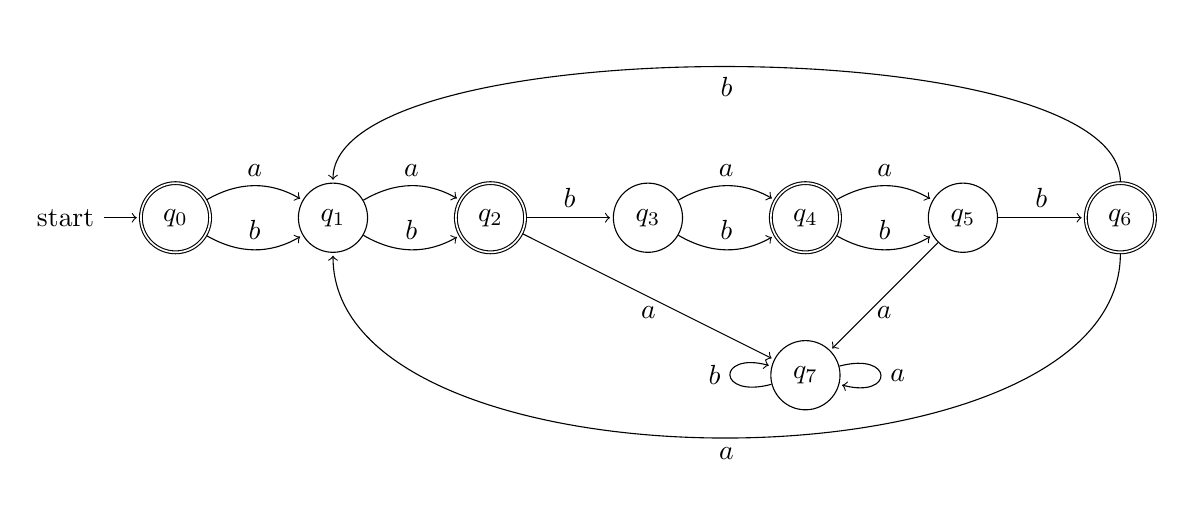
\begin{tikzpicture}[shorten >=1 pt, node distance =2 cm, on
grid, auto]
\node [state, initial, accepting] (q_0) {$ q_0$};
\node [state] (q_1) [right = of q_0] {$q_1$};
\node [state, accepting] (q_2) [right = of q_1] {$q_2$};
\node [state] (q_3) [right = of q_2] {$q_3$};
\node [state, accepting] (q_4) [right = of q_3] {$q_4$};
\node [state] (q_5) [right = of q_4] {$q_5$};
\node [state, accepting] (q_6) [right = of q_5] {$q_6$};
\node [state] (q_7) [below = of q_4] {$q_7$};
\path [->]
(q_0) edge [bend left] node {$a$} (q_1)
edge [bend right] node {$b$} (q_1)
(q_1) edge [bend left] node {$a$} (q_2)
edge [bend right] node {$b$} (q_2)
(q_2) edge [below] node {$a$} (q_7)
edge node {$b$} (q_3)
(q_3) edge [bend left] node {$a$} (q_4)
edge [bend right] node {$b$} (q_4)
(q_4) edge [bend left] node {$a$} (q_5)
edge [bend right] node {$b$} (q_5)
(q_5) edge [below] node {$a$} (q_7)
edge node {$b$} (q_6)
(q_6) edge [bend left=90, looseness=0.8] node {$a$} (q_1)
edge [bend right=90, looseness=0.5] node {$b$} (q_1)
(q_7) edge [loop right] node {$a$} ()
edge [loop left] node {$b$} ();
\end{tikzpicture}


\subsection*{c.}
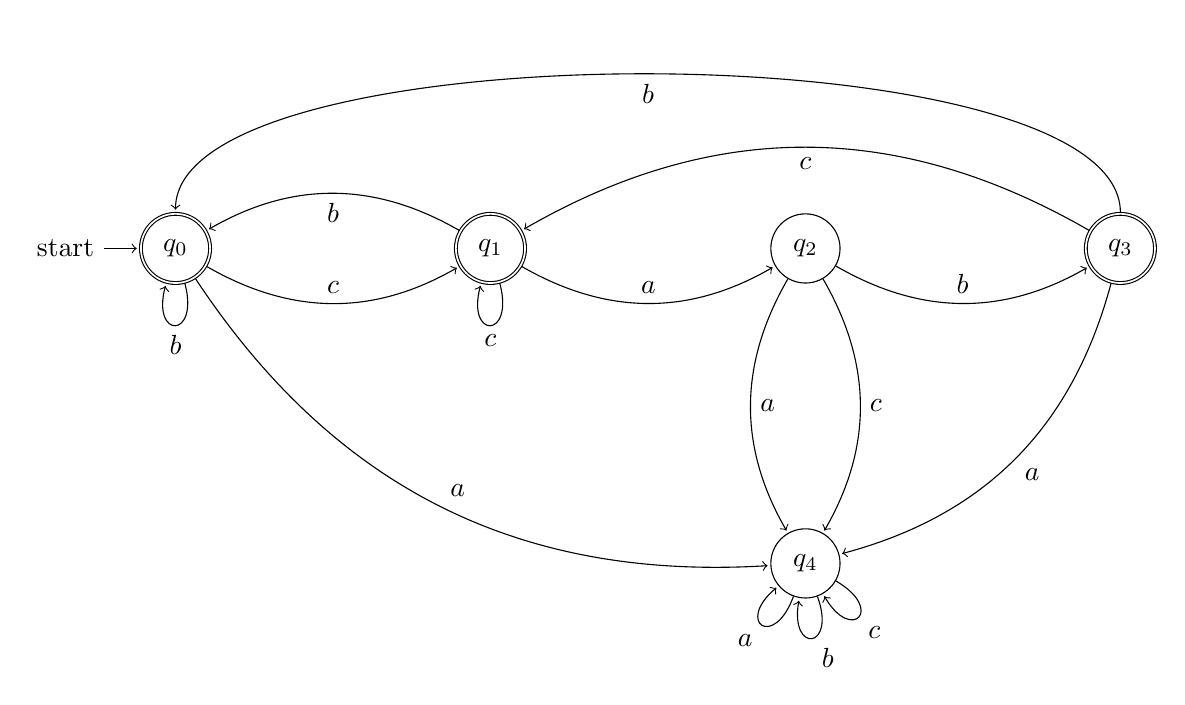
\begin{tikzpicture}[shorten >=1 pt, node distance =4 cm, on
grid, auto]
\node [state, initial, accepting] (q_0) {$ q_0$};
\node [state, accepting] (q_1) [right = of q_0] {$q_1$};
\node [state] (q_2) [right = of q_1] {$q_2$};
\node [state, accepting] (q_3) [right = of q_2] {$q_3$};
\node [state] (q_4) [below = of q_2] {$q_4$};
\path [->]


(q_0) edge [bend right] node {$a$} (q_4)
edge [loop below] node {$b$} ()
edge [bend right] node {$c$} (q_1)

(q_1) edge [bend right] node {$a$} (q_2)
edge [bend right] node {$b$} (q_0)
edge [loop below] node {$c$} ()

(q_2) edge [bend right] node {$a$} (q_4)
edge [bend right] node {$b$} (q_3)
edge [bend left] node {$c$} (q_4)

(q_3) edge [bend left] node {$a$} (q_4)
edge [bend right=90, looseness = 0.5] node {$b$} (q_0)
edge [bend right] node {$c$} (q_1)

(q_4) edge [in=220, out=250, loop] node {$a$} (q_4)
edge [in=260, out=290, loop] node {$b$} ()
edge [in=300,out=330, loop] node {$c$} ();


\end{tikzpicture}


\section*{Answer 3}

\subsection*{a.} The following is the computation tree for the string $abbb$ applied to given NFA $N$.

\begin{tikzpicture}[
  level distance=2cm,
  level 1/.style={sibling distance=(\textheight - 3cm)/2},
  level 2/.style={sibling distance=(\textheight - 3cm)/4},
  level 3/.style={sibling distance=(\textheight - 3cm)/4},
  level 4/.style={sibling distance=(\textheight - 3cm)/8},
  level 5/.style={sibling distance=(\textheight - 3cm)/8},
  level 6/.style={sibling distance=(\textheight - 3cm)/8}
  ]
  \node {$(q_0, abbb)$}
    child {node {$(q_1, bbb)$}
      child {node {$(q_2, bbb)$}}
      child {node {$(q_3, bbb)$}
        child {node {$(q_3, bb)$}
            child {node {$(q_3, b)$}
                child {node {$(q_3, e)$}}
                child {node {$(q_4, e)$}}}
            child {node {$(q_4, b)$}
                child {node {$(q_3, e)$}}}}
        child {node {$(q_4, bb)$}
            child {node {$(q_3, b)$}
                child {node {$(q_3, e)$}}
                child {node {$(q_4, e)$}}}}}
    }
    child {node {$(q_2, abbb)$}
      child {node {$(q_2, bbb)$}}
      child {node {$(q_4, bbb)$}
        child {node {$(q_3, bb)$}
            child {node {$(q_3, b)$}
                child {node {$(q_3, e)$}}
                child {node {$(q_4, e)$}}}
            child {node {$(q_4, b)$}
                child {node {$(q_3, e)$}}}}}
    };
\end{tikzpicture}
On the computation tree, it can be observed that none of the configurations lead to an accepting state as $q_3, q_4 \notin F$. Since a string is accepted by a nondeterministic finite automata if and only if there is at least one sequence of moves leading to a final step, is follows that $abbb \notin L(N)$.



\subsection*{b.}
\begin{equation}
    \begin{split}
        (q_0, ababa) & \vdash_{M} (q_1, baba) \\
        & \vdash_{M} (q_3, baba) \\
        & \vdash_{M} (q_3, aba) \\
        & \vdash_{M} (q_1, ba) \\
        & \vdash_{M} (q_3, ba) \\
        & \vdash_{M} (q_4, a) \\
        & \vdash_{M} (q_5, e)
    \end{split}
\end{equation}
Since a string is accepted by a nondeterministic finite automata if and only if there is at least one sequence of moves leading to a final step, it follows that $ababa \in L(N)$.




\section*{Answer 4}

\subsection*{a.}
Generalize Finite Automaton $M = (K_G, \Sigma_G, \Delta_G, s_G, F_G)$ satisfying $L(M) = L(N)$ is formally defined as follows,
\begin{itemize}
	\item $K_G = K \cup \{q_4\} \cup \{q_5\}$
	\item $\Sigma_G = \Sigma \cup R_0$ where $R_0$ is a finite subset of $R$ over $\Sigma$
	\item $\Delta_G \subseteq K \times (\Sigma_G \cup \{e\} \cup R) \times K$
	\item $s_G = q_4$
	\item $F_G = \{q_5\}$
\end{itemize}

$M$ can be shown graphically as follows,

\begin{tikzpicture}[shorten >=1 pt, node distance =4 cm, on
grid, auto]
\node [state, initial] (q_4) {$q_4$};
\node [state] (q_0) [right = of q_4] {$q_0$};
\node [state] (q_1) [above right = of q_0] {$q_1$};
\node [state] (q_2) [below right = of q_0] {$q_2$};
\node [state] (q_3) [below right = of q_1] {$q_3$};
\node [state, accepting] (q_5) [right = of q_3] {$q_5$};
\path [->]
(q_4) edge node {$e$} (q_0)
(q_0)edge [bend left] node {$b$} (q_1)
(q_1) edge [bend left] node {$a$} (q_2)
edge [bend left] node {$e$} (q_3)
(q_2) edge [bend left] node {$a$} (q_0)
edge [bend left] node {$b$} (q_1)
edge [in=255, out=285, loop] node {$b$} (q_2)
edge [bend right] node {$b$} (q_3)
edge [bend right] node {$e$} (q_5)
(q_3) edge [in=15, out=45, loop] node {$a$} (q_3)
edge node {$b$} (q_1)
edge node {$e$} (q_5);
\end{tikzpicture}

\subsection*{b.}

For this part we will start from the GFA defined in part a. and in each step apply the below equation and draw the obtained GFA.
\begin{equation}
	R(i, j, k) = R(i, j, k - 1) \cup R(i, k, k - 1)R(k, k,k - 1 )^{*}R(k, j, k - 1)
\end{equation}
Note that for the sake of simplicity, we will apply this equation only to those whose results are not empty set.


Eliminating $q_0$:

\begin{equation*}
	\begin{split}
		R(4, 1, 0) & = R(4, 1, -1) \cup R(4, 0, -1)R(0, 0, -1)^{*}R(0, 1, -1) = \emptyset \cup e \emptyset^* b = b \\
		R(2, 1, 0) & = R(2, 1, -1) \cup R(2, 0, -1)R(0, 0, -1)^{*}R(0, 1, -1) = b \cup a \emptyset^* b = b \cup ab
	\end{split}
\end{equation*}

\begin{tikzpicture}[shorten >=1 pt, node distance =4 cm, on
grid, auto]
\node [state, initial] (q_4) {$q_4$};
\node [state] (q_1) [above right = of q_4] {$q_1$};
\node [state] (q_3) [below right = of q_1] {$q_3$};
\node [state] (q_2) [below left = of q_3] {$q_2$};
\node [state, accepting] (q_5) [right = of q_3] {$q_5$};
\path [->]
(q_4)edge [bend left] node {$b$} (q_1)
(q_1) edge [bend left] node {$a$} (q_2)
edge [bend left] node {$e$} (q_3)
(q_2)edge [in=255, out=285, loop] node {$b$} (q_2)
edge [bend left] node {$b \cup ab$} (q_1)
edge [bend right] node {$b$} (q_3)
edge [bend right] node {$e$} (q_5)
(q_3) edge [in=15, out=45, loop] node {$a$} (q_3)
edge node {$b$} (q_1)
edge node {$e$} (q_5);
\end{tikzpicture}


Eliminating $q_1$:

\begin{equation*}
	\begin{split}
		R(4, 3, 1) & = R(4, 3, 0) \cup R(4, 1, 0)R(1, 1, 0)^{*}R(1, 3, 0) = \emptyset \cup b \emptyset^* e = b \\
		R(4, 2, 1) & = R(4, 2, 0) \cup R(4, 1, 0)R(1, 1, 0)^{*}R(1, 2, 0) = \emptyset \cup b \emptyset^* a = ba \\
		R(3, 3, 1) & = R(3, 3, 0) \cup R(3, 1, 0)R(1, 1, 0)^{*}R(1, 3, 0) = a \cup b \emptyset^* e = a \cup b \\
		R(3, 2, 1) & = R(3, 2, 0) \cup R(3, 1, 0)R(1, 1, 0)^{*}R(1, 2, 0) = \emptyset \cup b \emptyset^* a = ba \\
		R(2, 3, 1) & = R(2, 3, 0) \cup R(2, 1, 0)R(1, 1, 0)^{*}R(1, 3, 0) = b \cup (b \cup ab) \emptyset^* e = b \cup ab \\
		R(2, 2, 1) & = R(2, 2, 0) \cup R(2, 1, 0)R(1, 1, 0)^{*}R(1, 2, 0) = b \cup (b \cup ab) \emptyset^* a = b \cup ba \cup aba
	\end{split}
\end{equation*}

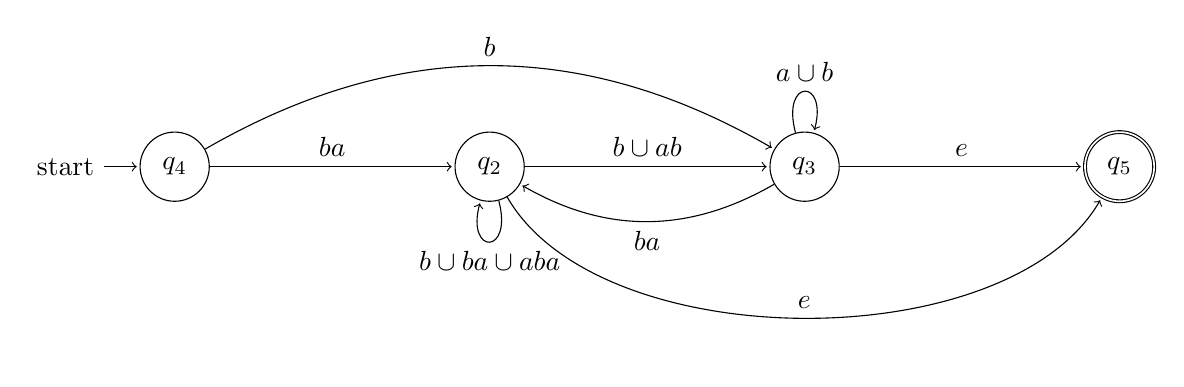
\begin{tikzpicture}[shorten >=1 pt, node distance =4 cm, on
grid, auto]
\node [state, initial] (q_4) {$q_4$};
\node [state] (q_2) [right = of q_4] {$q_2$};
\node [state] (q_3) [right = of q_2] {$q_3$};
\node [state, accepting] (q_5) [right = of q_3] {$q_5$};
\path [->]
(q_4)edge [bend left] node {$b$} (q_3)
edge node {$ba$} (q_2)
(q_2) edge [in=255, out=285, loop] node {$b \cup ba \cup aba$} (q_2)
edge node {$b \cup ab$} (q_3)
edge [bend right=60, looseness=0.8] node {$e$} (q_5)
(q_3) edge [in=75, out=105, loop] node {$a \cup b$} (q_3)
edge [bend left] node {$ba$} (q_2)
edge node {$e$} (q_5);
\end{tikzpicture}

Eliminating $q_2$:

\begin{equation*}
	\begin{split}
		R(4, 3, 2) & = R(4, 3, 1) \cup R(4, 2, 1)R(2, 2, 1)^{*}R(2, 3, 1) = b \cup ba(b \cup ba \cup aba)^*(b \cup ab) \\
		R(4, 5, 2) & = R(4, 5, 1) \cup R(4, 2, 1)R(2, 2, 1)^{*}R(2, 5, 1) = \emptyset \cup ba(b \cup ba \cup aba)^*e = ba(b \cup ba \cup aba)^* \\
		R(3, 3, 2) & = R(3, 3, 1) \cup R(3, 2, 1)R(2, 2, 1)^{*}R(2, 3, 1) = a \cup b \cup ba(b \cup ba \cup aba)^*(b \cup ab) \\
		R(3, 5, 2) & = R(3, 5, 1) \cup R(3, 2, 1)R(2, 2, 1)^{*}R(2, 5, 1) = e \cup ba(b \cup ba \cup aba)^*e = e \cup ba(b \cup ba \cup aba)^*
	\end{split}
\end{equation*}

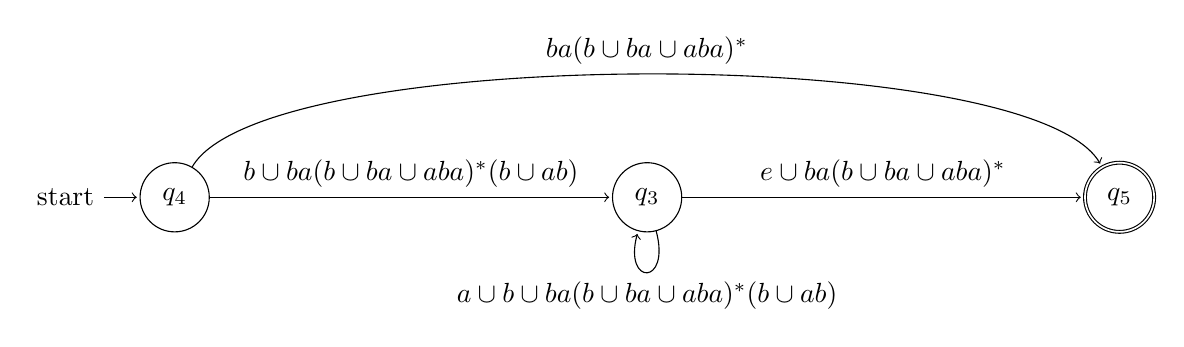
\begin{tikzpicture}[shorten >=1 pt, node distance =6 cm, on
grid, auto]
\node [state, initial] (q_4) {$q_4$};
\node [state] (q_3) [right = of q_4] {$q_3$};
\node [state, accepting] (q_5) [right = of q_3] {$q_5$};
\path [->]
(q_4)edge node {$b \cup ba(b \cup ba \cup aba)^*(b \cup ab)$} (q_3)
edge [bend left=60, looseness=0.4] node {$ba(b \cup ba \cup aba)^*$} (q_5)
(q_3) edge [in=255, out=285, loop] node {$a \cup b \cup ba(b \cup ba \cup aba)^*(b \cup ab)$} (q_3)
edge node {$e \cup ba(b \cup ba \cup aba)^*$} (q_5);
\end{tikzpicture}

Eliminating $q_3$:

\begin{equation*}
	\begin{split}
		R(4, 5, 2) & = R(4, 5, 2) \cup R(4, 3, 2)R(3, 3, 2)^{*}R(3, 5, 2) \\
		& = \big(ba(b \cup ba \cup aba)^*\big) \cup \big(b \cup ba(b \cup ba \cup aba)^*(b \cup ab)\big) \\ 
		& \qquad \big(a \cup b \cup ba(b \cup ba \cup aba)^*(b \cup ab)\big)^*\big(e \cup ba(b \cup ba \cup aba)^*\big)
	\end{split}
\end{equation*}

\begin{center}
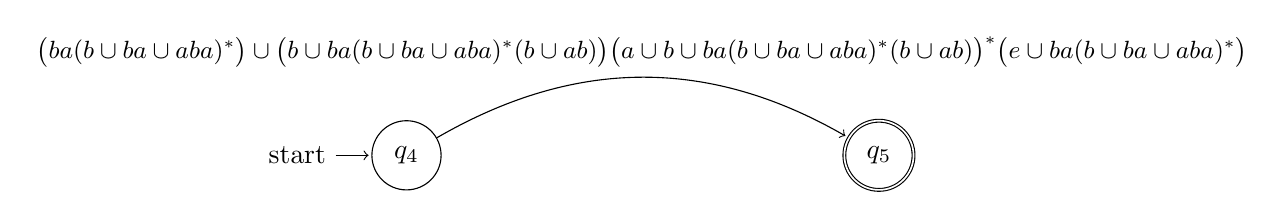
\begin{tikzpicture}[shorten >=1 pt, node distance =6 cm, on
grid, auto]
\node [state, initial] (q_4) {$q_4$};
\node [state, accepting] (q_5) [right = of q_4] {$q_5$};
\path [->]
(q_4) edge [bend left] node {\small $\big(ba(b \cup ba \cup aba)^* \big) \cup \big(b \cup ba(b \cup ba \cup aba)^*(b \cup ab)\big)\big(a \cup b \cup ba(b \cup ba \cup aba)^*(b \cup ab)\big)^*\big(e \cup ba(b \cup ba \cup aba)^*\big)$} (q_5);
\end{tikzpicture}
\end{center}

Hence, the regular expression obtained by state elimination is as follows,
\begin{equation*}
	\big(ba(b \cup ba \cup aba)^* \big) \cup \big(b \cup ba(b \cup ba \cup aba)^*(b \cup ab)\big)\big(a \cup b \cup ba(b \cup ba \cup aba)^*(b \cup ab)\big)^*\big(e \cup ba(b \cup ba \cup aba)^*\big).
\end{equation*}







\section*{Answer 5}

\subsection*{a.} Let's apply the subset construction algorithm on the given NFA $N$ in order to find the DFA $M = (K', \Sigma, \delta', s', F')$ such that $L(M) = L(N)$. By the algorithm, $K' = 2^K$ but since most of the states will not be reachable from the initial state $s'$, there is no need to consider all of them, so we are going to introduce a new state when it is needed during to construction. The definition of the function $E$ borrowed from the book (Elements of Theory of Computation), that is for any state $q \in K$, $E(q) = \{p \in K : (q, e) \vdash_{M}^{*} (p, e)\}$.\\

For the initial state $s'$ of $M$,
\begin{equation*}
    \begin{split}
        s' & = E(q_0)\\
        s' & = \{q_0, q_1, q_2\}
    \end{split}
\end{equation*}
Now we will find the transition function $\delta'$ by applying the following, for each $Q \subseteq K$ and each symbol $\alpha \in \Sigma$,
\begin{equation*}
    \begin{split}
        \delta'(Q, \alpha) & = \bigcup \{E(p) : p \in K \ and \ (q, a, p) \in \Delta \ for \ some \ q \in Q\} \\
    \end{split}
\end{equation*}
It follows that,
\begin{equation*}
    \begin{split}
        \delta'(s', a) & = \delta'(\{q_0, q_1, q_2\}, a) = E(q_1) \cup E(q_3) = \{q_1, q_3\} \\
        \delta'(s', b) & = \delta'(\{q_0, q_1, q_2\}, b) = E(q_2) = \{q_2\} \\
        \delta'(\{q_1, q_3\}, a) & = \emptyset \\
        \delta'(\{q_1, q_3\}, b) & = E(q_1) = \{q_1\} \\
        \delta'(\{q_2\}, a) & = E(q_3) = \{q_1, q_3\} \\
        \delta'(\{q_2\}, b) & = \emptyset \\
        \delta'(\{q_1\}, a) & = \emptyset \\
        \delta'(\{q_1\}, b) & = \emptyset \\
        \delta'(\emptyset, a) & = \emptyset \\
        \delta'(\emptyset, b) & = \emptyset
    \end{split}
\end{equation*}
$F'$ is the set of final states, it contains each set of states in which $q_3$ is a member, since $q_3$ is the only member of $F$; so among reachable states, that have been constructed above, $\{q_1, q_3\}$ is the only final state of $M$. Thus for $F'$, it follows that,
\begin{equation*}
    \begin{split}
        F' = \{\{q_1, q_3\}\}
    \end{split}
\end{equation*}
Hence, by applying construction algorithm on the NFA $N$, the DFA $M = (K', \Sigma, \delta', s', F')$ has been found such that $L(M) = L(N)$. \\
$M = (K', \Sigma, \delta', s', F')$ where,
\begin{equation*}
    \begin{split}
        K' & = \{\{q_0, q_1, q_2\}, \{q_1, q_3\}, \{q_2\}, \{q_1\}, \emptyset\}\\
        \Sigma & = \{a, b\} \\
        s' & = \{q_0, q_1, q_2\} \\
        F' & = \{\{q_1, q_3\}\}
    \end{split}
\end{equation*}
and $\delta'$ is given by the following table,
\begin{center}
    \begin{tabular}{c | c | c}
    \hline
        $q$ & $\sigma$ & $\delta'(q, \sigma)$ \\
        \hline
        $\{q_0, q_1, q_2\}$ & $a$ & $\{q_1, q_3\}$ \\
        $\{q_0, q_1, q_2\}$ & $b$ & $\{q_2\}$ \\
        $\{q_1, q_3\}$ & $a$ & $\emptyset$ \\
        $\{q_1, q_3\}$ & $b$ & $\{q_1\}$ \\
        $\{q_2\}$ & $a$ & $\{q_1, q_3\}$ \\
        $\{q_2\}$ & $b$ & $\emptyset$ \\
        $\{q_1\}$ & $a$ & $\emptyset$ \\
        $\{q_1\}$ & $b$ & $\emptyset$ \\
        $\emptyset$ & $a$ & $\emptyset$ \\
        $\emptyset$ & $b$ & $\emptyset$
    \end{tabular}
\end{center}

$M = (K', \Sigma, \delta', s', F')$ can be shown graphically as follows,

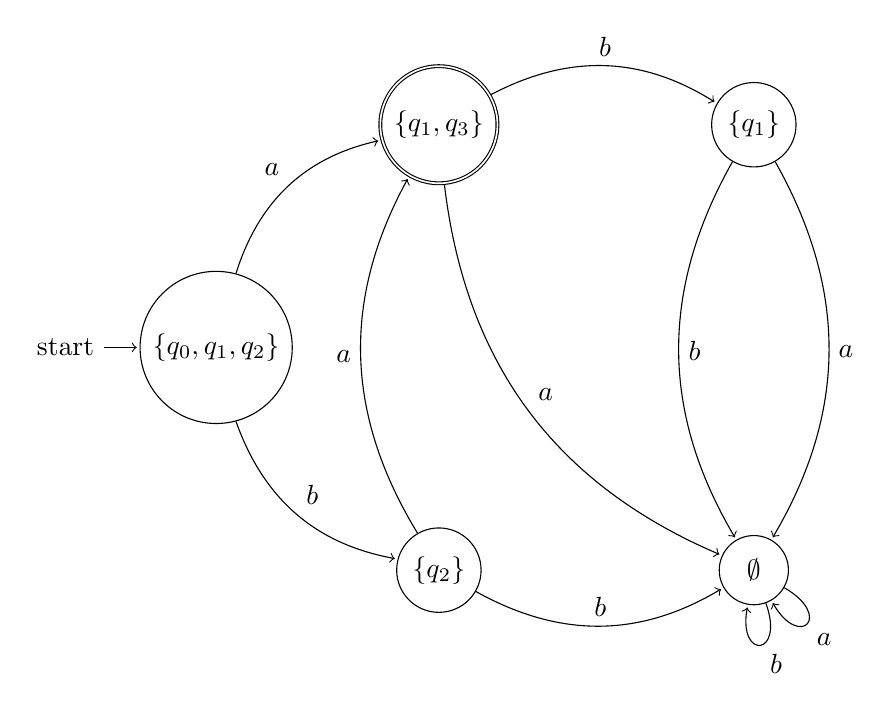
\begin{tikzpicture}[shorten >=1 pt, node distance =4 cm, on
grid, auto]
\node [state, initial] (q_0) {$\{q_0, q_1, q_2\}$};
\node [state, accepting] (q_1) [above right = of q_0] {$\{q_1, q_3\}$};
\node [state] (q_2) [below right = of q_0] {$\{q_2\}$};
\node [state] (q_3) [right = of q_1] {$\{q_1\}$};
\node [state] (q_4) [right = of q_2] {$\emptyset$};
\path [->]
(q_0) edge [bend left] node {$a$} (q_1)
edge [bend right] node {$b$} (q_2)
(q_1) edge [bend right] node {$a$} (q_4)
edge [bend left] node {$b$} (q_3)
(q_2) edge [bend left] node {$a$} (q_1)
edge [bend right] node {$b$} (q_4)
(q_3) edge [bend left] node {$a$} (q_4)
edge [bend right] node {$b$} (q_4)
(q_4) edge [in=300, out=330, loop] node {$a$} (q_4)
edge [in=260, out=290, loop] node {$b$} ();


\end{tikzpicture}

\subsection*{b.}
In part a, it has been proven that $L(M) = L(N)$ so it follows that $L = L(M) = L(N)$. Then $L$ is the language recognized by the DFA $M = (K', \Sigma, \delta', s', F')$ defined in part a. The complement of the language $\overline{L} = \Sigma^* - L(M)$ is accepted by the DFA $\overline{M} = (K', \Sigma, \delta', s', K' - F')$. That is, $\overline{M}$ is identical the M except its final and nonfinal states are swapped.

Regular expression for $\overline{L}$ can be expressed as follows,
\begin{equation*}
    \begin{split}
         e \cup b \cup bb(a \cup b)^* \cup ba(a \cup b)(a \cup b)^* \cup a(a \cup b)(a \cup b)^*
    \end{split}
\end{equation*}

$\overline{L}$ can be denoted using set notation as follows,
\begin{equation*}
    \begin{split}
         \overline{L} = \{w \in \{a, b\}^* : w \neq a \ \text{and} \ w \neq ba\}
    \end{split}
\end{equation*}



\section*{Answer 6}
Let $M_1 = (K_1, \Sigma, \delta_1, s_1, F_1)$ and $M_2 = (K_2, \Sigma, \delta_2, s_2, F_2)$ be deterministic finite automata such that $L_1 = L(M_1)$ and $L_2 = L(M_2)$. We shall construct a deterministic finite automaton $M = (K, \Sigma, \delta, s, F)$ such that $L(M) = L_1 - L_2 = L(M_1) - L(M_2) = L(M_1 - M_2)$. Note that, by definition every DFA is also a NFA so proposing an algorithm that constructs a DFA is the same as proposing an algorithm that constructs a NFA. Also every NFA can be converted into its equivalent DFA by applying subset construction algorithm. Thus, proposing an algorithm for one does not affect the generality of the proof. Formally, we define $M$ as follows,

$M = (K, \Sigma, \delta, s, F)$, where,

\begin{itemize}
        \item $K = K_1 \times K_2$
        \item $\Sigma \text{ is the same}$
        \item $\delta: (K_1 \times K_2) \times \Sigma \rightarrow (K_1 \times K_2), \text{ such that } \delta((p, q), \alpha) = (\delta_1(p ,\alpha), \delta_2(q, \alpha)), \text{ for } p \in K_1, \ q \in K_2 \text{ and } \alpha \in \Sigma$
        \item $s = (s_1, s_2)$
        \item $F = F_1 - F_2$
\end{itemize}
That is, the set of states $K$ contains the pairs from the Cartesian product of the $K_1$ and $K_2$. The alphabet $\Sigma$ is the same. The transition function $\delta$ is defined as $\delta((p, q), \alpha) = (\delta_1(p ,\alpha), \delta_2(q, \alpha))$ for $p \in K_1$, $q \in K_2$, and $\alpha \in \Sigma$. The initial state $s$ is the pair containing $s_1$ as its first member and $s_2$ as its second member. The set of accepting states $F$ contains the states that are in $F_1$ but not $F_2$, since the automaton $M$ accepts the language $L_1 = L(M_1)$ but does not accept the language $L_2 = L(M_2)$.

By the given algorithm above, given two arbitrary languages $L_1$ and $L_2$, we can construct a DFA (also a NFA) $M = (K, \Sigma, \delta, s, F)$ such that $L(M) = L_1 - L_2$. A language is regular if and only if it is accepted by a finite automaton (Theorem 2.3.2, Elements of Theory of Computation). From the if part of this theorem, the language $L(M) = L_1 - L_2$ is a regular language since we explicitly showed how to construct a FA accepting $L(M) = L_1 - L_2$. Hence, it has been proven that the class of regular languages is closed under set difference operation.



\section*{Answer 7}

\subsection*{a.}

Assume that $L$ is a regular language. Then by Pumping Lemma, there is an integer $n \geq 1$ such that any string $w \in L$ with $|w| \geq n$ can be rewritten as $w = xyz$ such that $y \neq e$, $|xy| \leq n$, and $xy^iz \in L$ for each $i \geq 0$.

\begin{equation*}
	L = \{w \in \{a, b\}^*: f(a, w) = n^2\text{ for some }n \in \mathbf{N}\}
\end{equation*}
In other words, for all $w \in L$, square root of the number of $a$ symbols in $w$ must be a natural number, so the distinctive feature of the strings focus on the symbol $a$. Thus, we are not interested in the number of $b$ symbols and their positions in $w$, so for the rest of the proof, without loss of generality, we will only consider strings which contain $a$ symbols.

Choose some $w \in L$ with $w = aaaa....aaaa$ and $|w| = m$ where $m = n^2$.

$w = aaaa....aaaa = xyz$ and $|xy| \leq n$ and $|y| = t$. Since $y \neq e$, $t \geq 1$.

Thus,
\begin{equation*}
	|xyz| = |xz| + |y| = (n^2 - t) + (t)
\end{equation*}

By Pumping Lemma, as $xyz \in L$, then $xy^iz \in L$ for each $i \geq 0$. Hence, $xy^2z \in L$ must be true.
\begin{equation*}
	|xy^2z| = |xz| + |y^2| = |xz| + 2|y| = (n^2 - t) + (2t) = n^2 + t
\end{equation*}

Since $|y| = t$ and $|xy| \leq n$, $t \leq n$. Thus,
\begin{equation*}
	n^2 + t \leq n^2 + n
\end{equation*}

Since $n \geq 1$,
\begin{equation*}
	\begin{split}
		n^2 + t & \leq n^2 + n < n^2 + 2n + 1 \\
		n^2 + t & < n^2 + 2n + 1 \\
		n^2 + t & < (n + 1)^2 \\
	\end{split}
\end{equation*}

Since $t \geq 1$,
\begin{equation*}
	n^2 < n^2 + t < (n + 1)^2
\end{equation*}

Hence, $n^2 + t$ is not a perfect square, in other words there is no such $c \in \mathbf{N}$ that satisfies $n^2 + t = c^2$. Thus, $xy^2z \notin L$. This a contradiction; assumption is discharged, $L$ is not a regular language.

\end{document}
